\documentclass[utf8,usehyperref,12pt]{G7-32}
\usepackage[T2A]{fontenc}
\usepackage[utf8]{inputenc} %% ваша любимая кодировка здесь
\usepackage[russian]{babel} %% это необходимо для включения переносов
%\usepackage{float}
\usepackage{textcase} 
\usepackage{lastpage}
\usepackage[dvips]{graphicx}

%\graphicspath{{pictures/}}
\DeclareGraphicsRule{*}{eps}{*}{}
\TableInChaper % таблицы будут нумероваться в пределах раздела
\PicInChaper   % рисунки будут нумероваться в пределах раздела
\setlength\GostItemGap{2mm}% для красоты можно менять от~0мм
\renewcommand{\labelenumi}{\arabic{enumi}.} 

% Определяем заголовки для титульной страницы
\NirOrgLongName{
Министерство общего и профессионального образования РФ

\MakeUppercase{Санкт-петербургский государственный университет информационных технологий, механики и оптики}
}
%\NirBoss{Научный руководитель}{И.И.Упырёв} %% Заказчик, утверждающийНИР
\NirManager{Научный руководитель}{Р.~В.~Иванов} 

\NirYear{2010}%% если нужно поменять год отчёта; если закомментировано, ставитсятекущий год
\NirTown{г. Санкт-Петербург,} %% город, в котором написан отчёт
% по проекту \No8550: 

% \NirIsAnnotacion{АННОТАЦИОННЫЙ } %% Раскомментируйте, если это аннотационный
%отчёт

\NirUdk{УДК \No 2123132123}
\NirGosNo{Регистрационный \No 123123}

%\NirStage{Этап \No 1.1}{промежуточный}{<<Обзор современного состояния торсионных
%наногенераторов>>} %%% Этап НИР: {номер этапа}{вид отчёта - промежуточный или
%заключительный}{название этапа}

\bibliographystyle{unsrt} %Стиль библиографических ссылок БибТеХа

%%%%%%%<------------- НАЧАЛО ДОКУМЕНТА
\begin{document}
\usefont{T2A}{ftm}{m}{} %%% Использование шрифтов Т2 для возможности скопировать
%текст из PDF-файлов.

\frontmatter %%% <-- это выключает нумерацию ВСЕГО; здесь начинаются
%ненумерованные главы типа Исполнители, Обозначения и~прочее

\NirTitle{\textbf{<<Выпускная квалификационная работа>>}}
%%% Название НИР и~генерация титульного листа


\Executors %% Список исполнителей здесь
%% это рисует линию размера 3мм и~толщиной 0.1 пункт
\begin{longtable}{p{0.35\linewidth}p{0.2\linewidth}p{0.35\linewidth}}
Научный руководитель, 	&		&	\\
Р.В.~Иванов	&\rule{1\linewidth}{0.1pt}	&  \\ \vspace{1cm}

Выполнил  &		&	\\
Н.В.~Назаренко, & \rule{1\linewidth}{0.1pt}& \\
\end{longtable}

\Referat %% Реферат отчёта, не~более 1 страницы
Отчёт \pageref{LastPage}~c. 4~рис., 3~табл.

\MakeUppercase{Linux, хранилилище, webdav}



%\tableofcontents

%\NormRefs % Нормативные ссылки 
%\Defines % Необходимые определения 
%СУБД -
%FUSE -


\Introduction

placeholder

\mainmatter %% это включает нумерацию глав и~секций в документе ниже

\chapter{Постановка задачи}
\section{Обзор особенностей заказчика}
\subsection{Организационная структура}
Санкт-петербургский городской дворец творчества юных(СпбГДТЮ) обладает большой и сложной организационной структурой, для каждого элемента которого, характерен свой вид деятельности. Рассмотрим организацию с точки зрения двух аспектов: территориального и структурного.

\begin{figure}[ht]
   \centering%центрируем картинку
   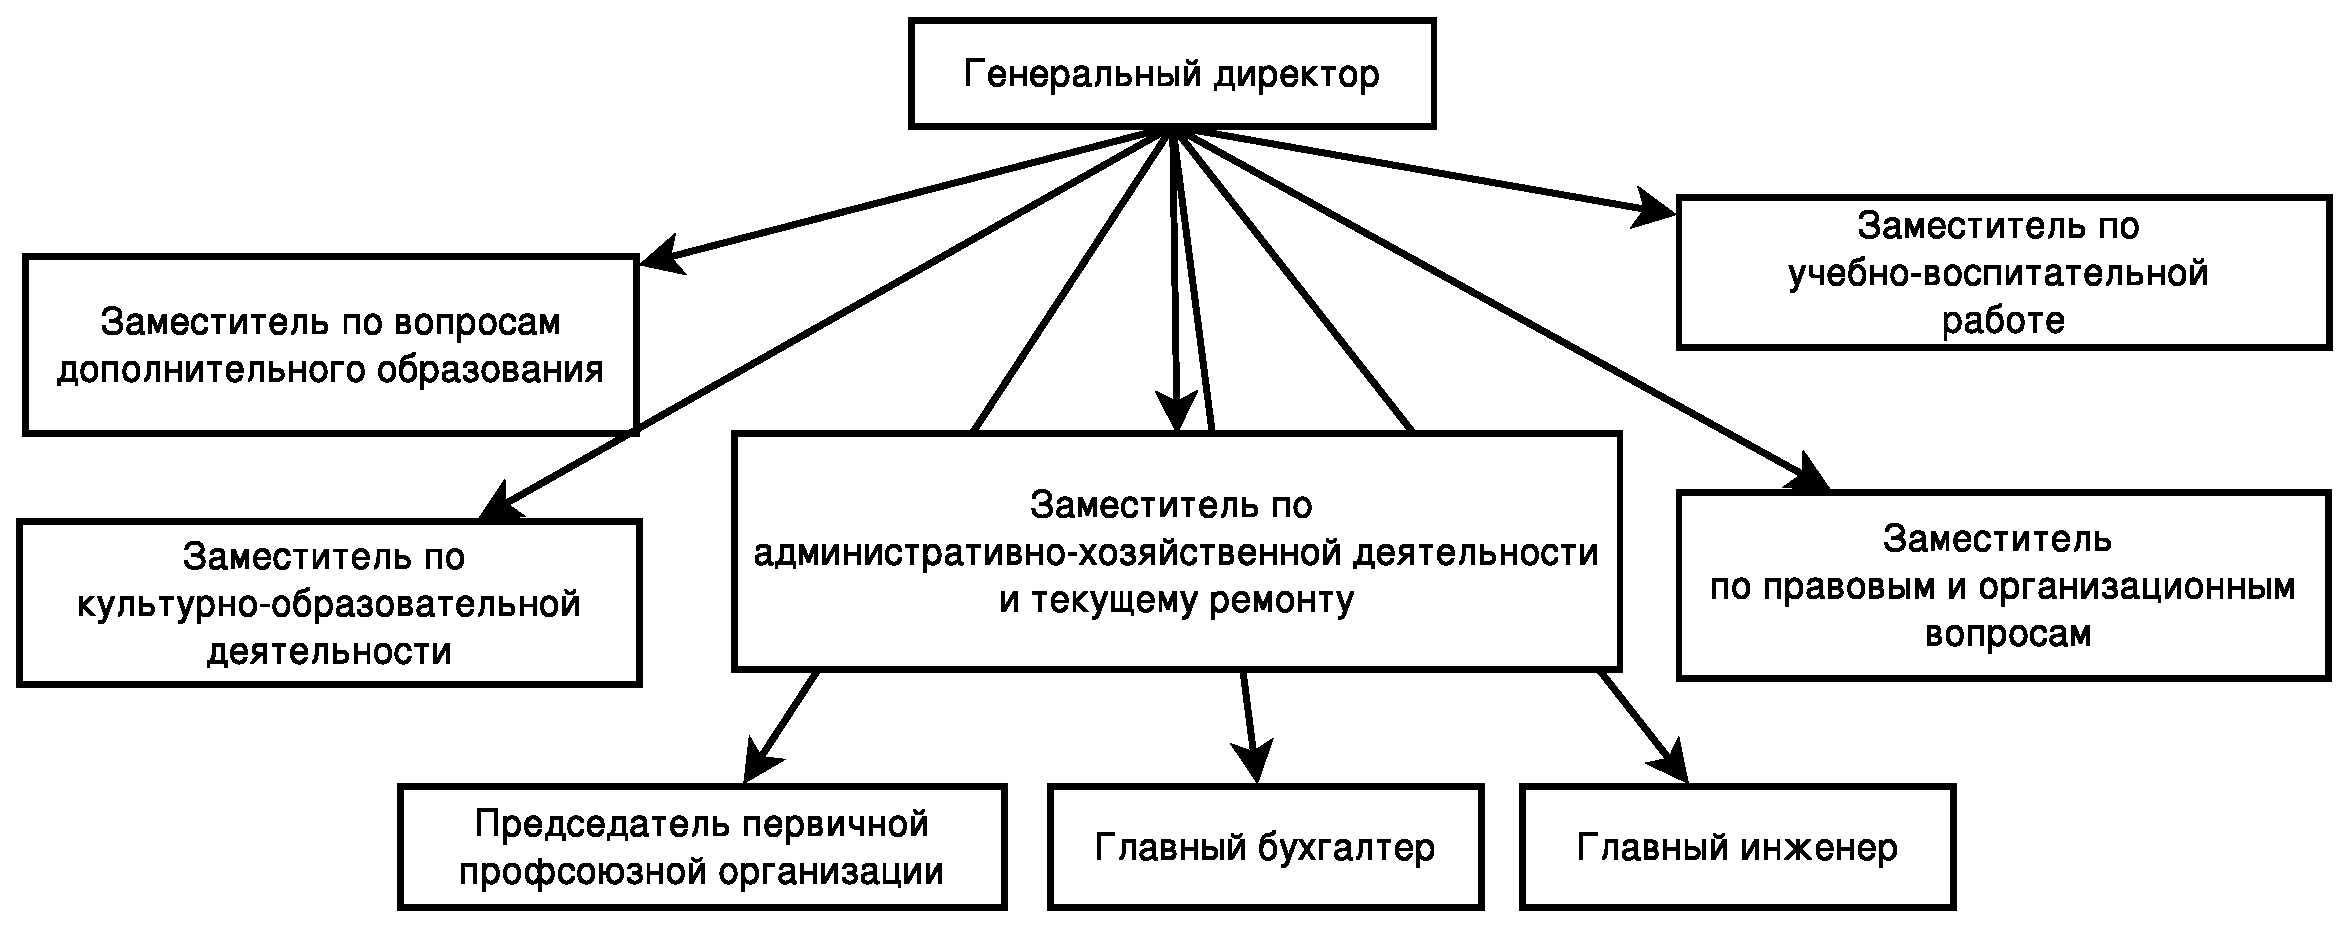
\includegraphics[height=160mm, width=0.8\textwidth, clip, keepaspectratio]{pictures/management_structure.eps}
   \caption{Структура управления организацией}\label{fig:fig_management_struct}
 \end{figure}

Территориальная распределенность обусловленна тем, что Дворец творчества юных расположен в центре города, на его территории находиться множество отдельных корпусов, а также ему принадлежит довольно большой участок земли на Крестовском острове и ЗЦДЮТ <<Зеркальный>>. Доступ пользователей к глобальным и локальным информационным ресурсам обеспечивается подключениями по выделенной линии
(2 мб/с), по оптоволокну (1000 мб/с) и прямыми подключениями к узлу (100 мб/с). Сеть рассчитана на большое количество пользователей ИТ-инфраструктурой (более
15 000 компьютеров). Среди них: работники дворца; педагоги; управляющий персонал;  персонал, отвечающий за сервисную деятельность; учащиеся. Сложность управленческой структуры организации определяется большим штатом сотрудников и широким спектром исполняемых функций. Главным руководителем является генеральный директор, которому подчиняются различные подразделения такие как: финансовый, хозяйственный, учебно-воспитательный и другие сектора.

\begin{figure}[ht]
   \centering%центрируем картинку
   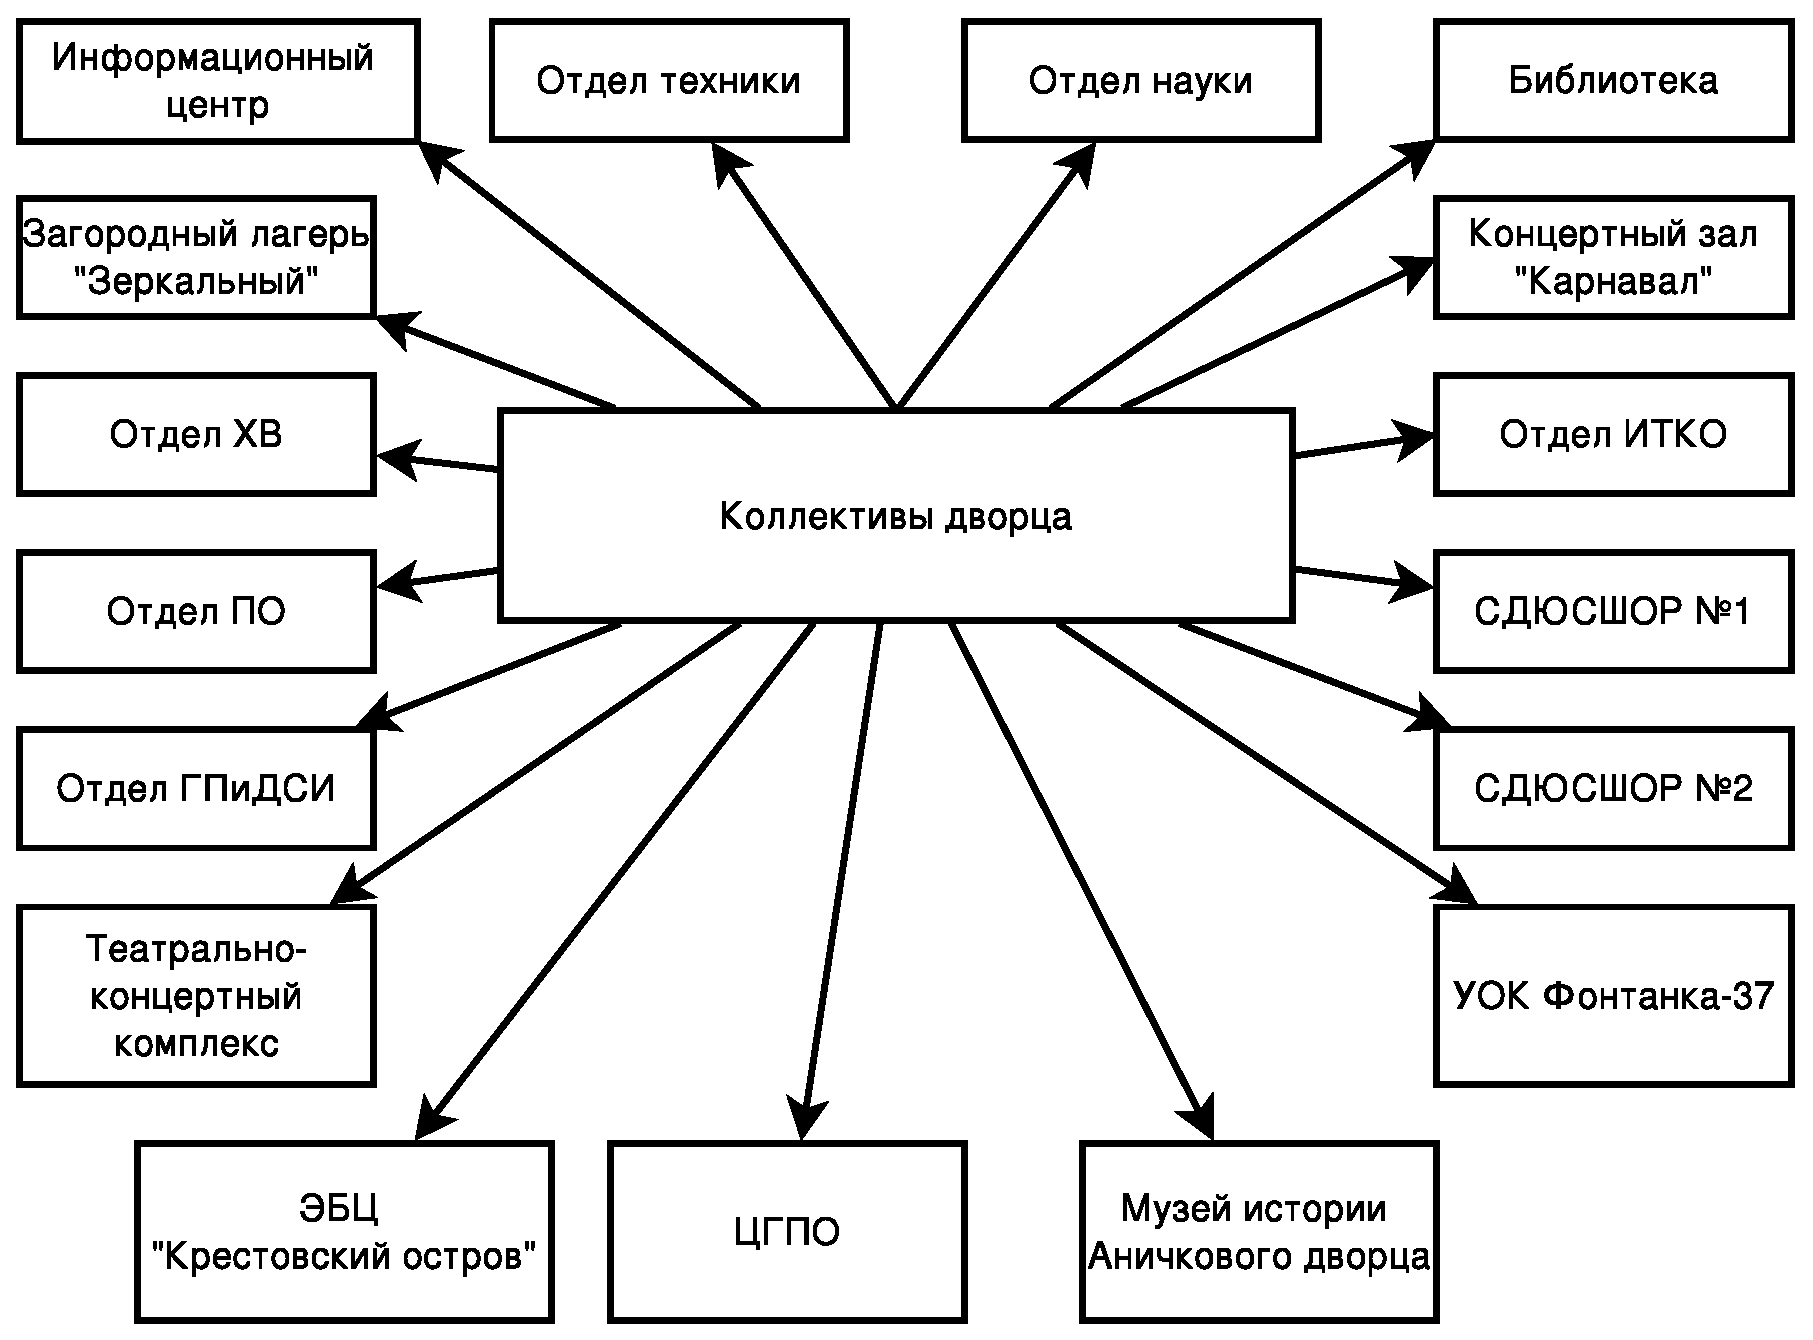
\includegraphics[height=160mm, width=0.8\textwidth, clip, keepaspectratio]{pictures/org_struct.eps}
   \caption{Структура подразделений}\label{fig:org_structure}
 \end{figure}

Сотрудники дворца разделены на коллективы или отделы, отвечающие за определенный вид деятельности(рисунок \ref{fig:org_structure}).
Каждый отдел в свою очередь имеет большое количество своих подразделений. У каждого коллектива или отдела есть свой директор, один или несколько заместителей и большое количество сотрудников.


\begin{itemize}
\item Отдел ХВ – отдел художественного воспитания
\item Отдел ПО – отдел предшкольного  образования
\item Отдел ГПиДСИ – отдел гуманитарных программ и детских социальных инициатив
\item Отдел ИТКО – отдел информационных технологий и компьютерного обеспечения
\item СДЮС школа №1 – специализированная детско-юношеская спортивная школа №1
\item СДЮС школа № – специализированная детско-юношеская спортивная школа №2
\item УОК <<фонтанка-37>> – учебно-оздоровительный комплекс <<фонтанка-37>>
\item ЭБЦ <<крестовский остров>> – эколого-биологический центр <<крестовский остров>>
\item ЦГПО – центр городских предметных олимпиад.
\end{itemize}

Основной функцией дворца является оказание образовательных и воспитательных услуг, которые оказывают учебные коллективы, осуществляющие свою деятельность под управлением методических подразделений самого Дворца
и управляющих организаций МОиН города. Кроме непосредственно обучения сотрудники  составляют различные учебные программы, рабочие планы, отчеты, разрабатывают учебно-методические пособия.
Обеспечением текущей деятельности дворца, в аспекте поддержания в надлежащем состоянии оборудования, коммуникаций занимаются сервисные подразделения Дворца. Схема должностей СПБГТЮ представлена на рисунке \ref{fig:fig_management_struct}.

\subsection{Задачи требующие инфраструктурного сопровождения}\label{ssect:tasks_infra}
Основной функцией дворца является оказание образовательных и воспитательных услуг, предоставление которых оказывают учебные коллективы, осуществляющие свою деятельность под управлением методических подразделений самого Дворца
и управляющих организаций МОиН города. Кроме непосредственно обучения сотрудники составляют различные учебные программы, рабочие планы, отчеты, разрабатывают учебно-методические пособия. 

Для обеспечения работы сотрудников требуется система сетевого хранения файлов по подразделениям с возможностью разделения прав доступа сотрудников. Такое разделение необходимо для того, чтобы . Для разных подразделений это могут быть различные виды файлов: изображения, документы в различных форматах, аудио или видео информация и так далее. Подразделениям необходима возможность выкладывать файлы в общий доступ.

\subsection{Ограничения накладываемые на информационное сопровождение}\label{ssect:restrict_infra}
Поскольку организация осуществляет переход на свободное программное обеспечение, то требуется использование исключительно свободных программных продуктов для реализации системы хрпнения файлов. В проекте используются только компоненты распространяющиеся под свободными лицензиями, одобренными OSI(Open Software Initiative). Решение должно функционировать в операционной системе GNU/Linux и быть независимым от ОС установленной на рабочем месте пользователя.

У педагогов в следствии недостатка времени и иногда отсутствия желания осваивать новый продукт могут возникнуть трудности при переходе на новую информационную систему. С другой стороны, педагоги – люди, которые умеют учиться, что является неоспоримым плюсом для более быстрого перехода на новую систему.

Кроме того, многие педагоги работают не только во Дворце, но и дома, где зачастую используется другое программное обеспечение, в большинстве случаев проприетарное. Следовательно, необходимо предоставить возможность доступа к служебной информации, методическим и др. материалам, необходимым для обеспечения профессиональной деятельности без привязки к определённым операционным системам.

Управленческий аппарат почти весь состоит из людей далёких от информационный технологий. У таких сотрудников нет желания менять устоявшийся бизнес-процесс, поэтому их приходиться заставлять переучиваться, используя административный ресурс, что накладывает жёсткие ограничения на сложность использования системы хранения файлов.

%Сервисные сотрудники обладают большим количеством свободного времени,
%но у них отсутствует желание работать, трудиться, им свойственна лень, поэтому им не хочется учиться, но процесс обучения у них происходит быстрее за счёт имеющихся знаний.

Во Дворце ежедневного находится большое количество сотрудников, выполняющих свои непосредственные обязанности, поэтому функционирование Дворца является непрерывным процессом, поэтому его не только не следует приостанавливать,
а категорически не рекомендуется это делать.

Таким образом система сетевого доступа к файлам должна быть максимально простой с точки зрения пользователя, использовать стандартизованные решения, реализации которых есть под все популярные операционные системы и быть открытым программным обеспечением.

\subsection{Предположительные архитектурные решения и задачи информационной системы}\label{ssect_arch_tasks}
Исходя из положений раздела~\ref{ssect:tasks_infra} задачей хранилища данных является хранение файлов пользователей, дерева каталогов, информации о пользователях и их правах доступа. В процессе работы, пользователи будут использовать большое количество различных форматов файлов, поэтому представление файла в системе хранения должно быть максимально обобщённым. 

Система ориентирована на пользователей с различным уровнем знакомства с информационными технологиями(раздел~\ref{ssect:restrict_infra}). Для минимизации риска утери данных при случайном удалении или перезаписи файлов требуется реализовать хранение истории версий таким образом, чтобы пользователь мог получить доступ к удалённому файлу или одной из предыдущих доступных версий. В то же время, для уменьшения обьёма данных хранящихся на жестком диске хранилища, требуется возможность окончательного удаления предыдущих версий файлов по прошествии определённого срока администратором системы.

Для осуществления контроля за действиями пользователей и поиска ошибок в работе системы требуется сохранять информацию о действиях пользователей в системе с момента входа в систему. Для поиска проблемы необходимо знать какие действия выполнял пользователь в указанный момент времени и были ли ему разрешены данные действия правами доступа на тот момент.

Для управления пользователями и правами доступа требуется отдельное приложение, позволяющее создавать, удалять изменять информацию о пользователях; создавать, редактировать, удалять подгруппы; управлять составом пользователей в группах и назначать права доступа к группам для пользователей.

Таким образом требуется:
\begin{itemize}
\item предоставление удобного доступа пользователя к файлам и директориям, на которые ему были установлены права доступа.
\item осуществление разделения пользователей по ролям доступа
\item хранение предыдущих версий файлов с возможностью их последующего удаления
\item ведение журнала активности пользователей
\end{itemize}

Исходя из требований к системе, предлагается трёхзвенная архитектура: Клиент -- сервер приложений -- хранилище данных. Такая архитектура позволяет разделить логику работы клиент-серверной части и хранения файлов в хранилище данных. 

\section{Обзор аналогов}\label{sect_analogs}
\subsection{Системы управления версиями}
Система управления версиями — программное обеспечение для облегчения работы с изменяющейся информацией. Система управления версиями позволяет хранить несколько версий одного и того же документа, при необходимости, возвращаться к более ранним версиям, определять, кто и когда сделал то или иное изменение и многое другое.

Системы контроля версий такие как: git, svn, cvs; требуют определённой подготовки от пользователя. Это решение требует от пользователя ручного получения файлов из хранилища и помещения их обратно. Исходя из причин по которым создавались такие системы, невозможно ограничить глубину сохранения версий файлов, что при использовании не-текстовых данных приводит к быстрому разрастанию хранилища файлов.

Решение на основе git является наиболее безопасным, поскольку все данные передаются через шифрованное соединение, а аутентификация пользователя производится на основе криптографических ключей.

\subsection{Системы электронного документооборота}
Система документооборота, система электронного документооборота (СЭД) — автоматизированная многопользовательская система, сопровождающая процесс управления работой иерархической организации с целью обеспечения выполнения этой организацией своих функций. При этом предполагается, что процесс управления опирается на человеко-читаемые документы, содержащие в слабо формализованной форме инструкции для сотрудников организации, необходимые к исполнению.

Такие системы ориентированы на управление бизнес-процессами и оперируют понятием документа. Организовать в такой системе совместную работу над разнородными материалами, такими как методические пособия сложно, поскольку зачастую это может быть мультимедийная информация к обработке и хранению которой СЭД не приспособлены.

\subsection{ownCloud}
ownCloud - облачное хранилище данных позволяющее получать доступ к данным.

Система поддерживает автоматическое резервное копирование, версионный контроль изменений и шифрование передачи данных. Доступ к хранилищу может быть обеспечен при помощи монтирования сетевого раздела, WebDAV, KDE KIO-Slaves, приложения для мобильных телефонов или через web-интерфейс. Данные также могут быть синхронизированы с локальной копией для последующего offline-использования. Исходные тексты системы распространяются в рамках лицензии AGPL.

Эта система нацелена на личное использование и не обладает требуемыми в разделе~\ref{ssect:restrict_infra} возможностями по организации доступа к файлам различных подразделений и пользователей.

\subsection{Выводы}

Из рассмотренных аналогов, требованиям раздела~\ref{ssect_arch_tasks} полностью не соответствует ни один представленных аналогов. Системы контроля версий требуют значительной начальной подготовки пользователей для работы с такой системой. Системы электронного документооборота изначально не предназначены для хранения мультимедийной информации. ownCloud не позволяет управлять разделением прав доступа в объёме требуемом согласно~\ref{ssect_arch_tasks}.

Таким образом для реализации поставленной задачи требуется разработать клиент-серверную систему, сочетающую в себе удобство доступа к файлам, широкие возможности по управлению правами доступа и управляемое версионное хранение файлов в хранилище.

\section{Формализация технического задания}
\subsection{Платформа}\label{ssect:platform}
Исходя из ограничений описанных в разделе~\ref{ssect:restrict_infra} требуется использование исключительно свободного ПО для реализации системы хранения файлов. 

Для работы системы используется операционная система GNU/Linux, в частности дистрибутив Ubuntu. Для работы системы на рабочем месте пользователя требуется наличие следующих библиотек:

\begin{itemize}
 \item neon - Библиотека реализующая протокол WebDAV на языке C. Лицензии: GPL, LGPL
 \item expat - Библиотека для работы с XML документами. Лицензия: MIT.
 \item fuse - Библиотека для разработки файловых систем в пространстве пользователя. Лицензия GPLv2.
 \item glibc - стандартная библиотека языка C. Лицензии: GPL, LGPL.
\end{itemize}

Для работы серверной части требуются следующие библиотеки:
\begin{itemize}
 \item psycopg2 - Интерфейс к СУБД PostgreSQL.
 \item sqlalchemy - Библиотека объектно-реляционного отображения данных.
\end{itemize}
Все указанные библиотеки распространяются под лицензиями одобренными организацией OSI. Такие лицензии позволяют неограниченное использование, распространение, изучение и модификацию исходных текстов библиотек и приложений, которые распространяются на условиях этих лицензий.

\subsection{Средства разработки}

Для разработки системы используются следующие программные продукты:
\begin{itemize}
 \item Eclipse -- свободная интегрированная среда разработки модульных кроссплатформенных приложений.
 \item pydev -- модуль для разработки и отладки для языка Python.
 \item CDT -- модуль для разработки и отладки для языков C и C++.
 \item Visual Paradigm Community Edition -- средство проектирования UML диаграмм.
 \item PostgreSQL -- свободная объектно-реляционная система управления базами данных (СУБД).  
\end{itemize}

Система основана на следующих открытых решениях:
\begin{itemize}
 \item pywebdav -- реализация WebDAV протокола на языке Python. Распространяется на условиях лицензии GPLv2.
 \item davfs2 -- реализация доступа к хранилищу данных с использованием WebDAV протокола. Представляет собой реализацию файловой системы в пространстве пользователя. Распространяется на условиях лицензии GPLv2.
\end{itemize}

Использование готовых решений позволяет значительно сократить затраты на разработку и отладку и тестирование системы. Исходя из проектов взятых за основу, в работе используются языки C и Python. 

Исходя из требований лицензии GPLv2 результат данной дипломной работы также распространяется по условиям лицензии GPLv2.

\subsection{Функциональные требования}\label{ssect_req}

Исходя из положений раздела~\ref{ssect_arch_tasks} и возможностей рассмотренных аналогов в разделе~\ref{sect_analogs} был сформулирован список требований к системе.

Требуется ведение журнала активности пользователей, включающего в себя информацию о следующих действиях: 
\begin{itemize}
\item дату и время входа/выхода пользователя
\item создание файла
\item модификация файла
\item удаление файла
\item установка блокировки на файл
\item снятие блокировки с файла
\end{itemize}

Требуется предоставить удобный доступ пользователя к файлам и директориям, на которые ему были установлены права доступа такие как: чтение, запись, удаление файлов и каталогов. Этот инструмент должен предоставлять возможность пользователю работать с хранилищем данных точно также, как и с локальной директорией. Это значит, что от пользователя не должно требоваться каких либо действий для сохранения данных в хранилище, кроме как ввод пользовательских данных при подключении к системе.

Для реализации поставленных условий требуется разработать инструмент позволяющий:	
\begin{itemize}
%\item получать информацию об изменениях произошедших с последнего входа пользователя в систему	
\item выполнять аутентификацию пользователя по логину/паролю	
\item выполнять подключение рабочей области пользователя в дерево каталогов
\end{itemize}

Необходимо осуществлять разделение пользователей по следующим ролям:	
\begin{itemize}
\item Пользователь 	в соответствие со своими правами имеет 	доступ к файлам и каталогам подразделения и к общим каталогам. Имеет доступ к предыдущим версиям своих файлов на чтение. 		
\item Администратор подразделения может назначать права доступа для сотрудников подразделения, создавать и удалять каталоги в каталоге подразделения. Имеет доступ на чтение к предыдущим версиям файлов подразделения	
\item Администратор создает и удаляет учётные записи пользователей, записи подразделений, назначает права доступа, имеет полный 	доступ к дереву каталогов, имеет полный 	доступ к предыдущим версиям файлов.
\end{itemize}

Требуется разработать инструмент для администраторов групп, для делегирования им прав на управление подгруппами, создание подгрупп, создание, модификацию и удаление пользователей и управление правами доступа пользователей к подгруппам.

\chapter{Проектирование}
\section{Системные архитектурные решения}
\subsection{Распределение задач между компонентами}

На основании требований в разделе~\ref{ssect:req} система состоит из следующих компонентов:
\begin{itemize}
\item пользовательское приложение;
\item серверная часть;
\item административный интерфейс;
\item хранилище данных;
\end{itemize}

Пользовательское приложение реализует сетевой доступ к файлам находящимся в хранилище, посредством WebDAV протокола. Задачами клиентской части являются:
\begin{itemize}
\item запрос учётных данных пользователя
\item реализация представления файловой системы и подключение её к дереву каталогов пользователя
\item реализацию протокола общения между клиентской частью и сервером приложений
\item передача файлов пользователя серверу приложений
\item получение запрошенных файлов с сервера приложений
\end{itemize}

Серверная часть реализует интерфейс между клиентским приложением и хранилищем данных. Также к серверной части относится административный интерфейс администратора.

В рамках серверной части обеспечивается:
\begin{itemize}
\item авторизация пользователей, 
\item предоставление требуемых файлов и каталогов для работы в соответствие с правами доступа, 
\item блокировка используемых файлов 
\item получение обновлённой версии с возможным получением предыдущих версий файла.
\item запись информации о действиях пользователей в рамках системы
 \end{itemize}
 
Административный интерфейс реализует следующие возможности:

\begin{itemize}
	\item создание и модификация учётных записей пользователей;
	\item создание и модификация групп пользователей;
	\item редактирование состава пользователей в группах и подгруппах;
	\item назначение прав доступа пользователей в группах;
\end{itemize}

Хранилище данных решает задачу хранения пользовательских данных, файлов, дерева каталогов и вспомогательных сущностей.

%\subsection{Описание задач решаемых отдельными компонентами}
%\subsection{Проектирование требований к физической и программной инфраструктуре}
% список ПО на компах
% для работы клиентского ПО требуется ....

\section{Архитектура программы}
\subsection{Архитектура клиентской части}

Клиентская часть реализует доступ к файловому хранилищу как к подкаталогу в дереве файлов пользователя. Это достигается использованием средств, которые позволяют предоставить POSIX интерфейс к сетевому хранилищу данных.

\begin{figure}[ht]
   \centering%центрируем картинку
   \includegraphics[height=160mm, width=0.8\textwidth, clip, keepaspectratio]{pictures/client_sequencs.eps}
   \caption{Схема взаимодействия клиента с сервером приложений}\label{fig:client_sequence}
 \end{figure}

На диаграмме последовательностей (рисунок \ref{fig:client_sequence}) показаны события происходящие в процессе работы пользователя с файловой системой. В работе пользователя выделяются три основных этапа: монтирование, изменение объектов файловой системы и отмонтирование системы. 

При монтировании ФС, у пользователя запрашивают его логин/пароль для работы в системе, после этого сервер приложений проверяет правильность введённых данных и аутентифицирует его и возвращает содержимое корневой директории пользователя.

При изменениии файла происходит блокировка ресурса на сервере приложений. Запись данных пользователем идёт в локальный кэш, который после закрытия файла отправляется на сервер приложений. Использование кеширования позволяет уменьшить количество версий файлов, особенно для приложений в которых используется автосохранение файлов.

При отсоединении происходит отправка данных из кеша клиентской части на сервер приложений и отключение от сервера приложений.

\subsection{Архитектура сервера приложений}

Сервер приложений используется для обработки запросов пользователей и подготовкой полученных файлов к сохранению в хранилище. Сервер приложений состоит из многопоточного обработчика запросов пользователей, обработчика аутентификации и авторизации пользователей и обработчика davfs протокола используемого для связи с клиентским приложением.

\begin{figure}[ht]
   \centering%центрируем картинку
   \includegraphics[height=160mm, width=0.8\textwidth, clip, keepaspectratio]{pictures/davstorage.eps}
   \caption{Диаграмма значимых классов проекта}\label{fig:davstorage}
 \end{figure}
 
 Диаграмма классов системы, без реализации WebDAV и http-сервера представлена на рисунке \ref{fig:davstorage}. Система постоена на принципе независимости от реализации хранения файлов и информации о пользователях, что позволяет реализовать своё хранилище данных, реализующее интерфейс для WebDAV протокола.
 
 %хранение данных в БД, помянуть про large objects

\subsection{Архитектура БД}

В проекте используется технология объектно-реляционного отображения, позволяющая работать с записями в БД, как с объектами языка программирования. Такой подход позволяет представить БД как абстрактное хранилище объектов и не задумываться над деталями конкретной реализации БД.

Для хранения данных может использоваться любая реляционная СУБД, которая поддерживается выбранной библиотекой для объектно-реляционного отображения.

\begin{figure}[ht]
   \centering%центрируем картинку
   \includegraphics[height=160mm, width=0.8\textwidth, clip, keepaspectratio]{pictures/DB.eps}
   \caption{Схема БД}\label{fig:db_scheme}
 \end{figure}

Основные сущности используемые в системе показаны на рисунке \ref{fig:db_scheme}. В БД хранится информация о пользователях, группах, правах доступа, хранящихся файлах их содержимом и версиях.


\section{Проектирование инфраструктуры}

\subsection{Оценка требований к рабочему месту пользователя}
Основные характеристики и конфигурация рабочего места пользователя:
\begin{itemize}
 \item Платформа x86
 \item Intel Celeron 1.7 GHz
 \item RAM 1 GB
 \item Жёсткий диск - 80 Гб
\end{itemize}

\subsection{Оценка требований к серверу}

Исходя из назначения системы, требуется особое внимание уделить дисковому хранилищу. Дисковое хранилище должно обеспечивать высокую отказоустойчивость и как можно меньшее время доступа к информации. Этими свойствами обладают массивы дисков RAID, в частности RAID5, которые позволяют эффективно использовать место на дисках массива.

Основные характеристики и конфигурация сервера:
\begin{itemize}
 \item Платформа x86
 \item Xeon 1.6 GHz
 \item RAM 2 GB
 \item Дисковый массив – 4 SATA диска объединенные в RAID 5, 4x400 GB
\end{itemize}

Требуемыми характеристиками обладает сервер HP ProLiant DL160 G6 производства компании Hewlett-Packard. Этот сервер также сертифицирован на полную совместимость с дистрибутивом Ubuntu и может быть рекомендован к использованию.

\subsection{Оценка требований к пропускной способности канала}
Для работы с сервером, клиенту требуется соединение с пропускной способностью 10 МБит/сек. Для сервера требуется соединение с пропускной способностью не менее 100 МБит/сек.

\chapter{Реализация}

\section{Особенности реализации клиентской части}
Клиентская часть состоит из модуля к FUSE, утилит монтирования и графического интерфейса для утилит монтирования для упрощения работы пользователям. 

\begin{figure}[ht]
   \centering%центрируем картинку
   \includegraphics[height=160mm, width=0.8\textwidth, clip, keepaspectratio]{pictures/fuse_structure.eps}
   \caption{Схема работы FUSE}\label{fig:fuse_structure}
 \end{figure}

Filesystem in Userspace (FUSE) (Файловая система в пользовательском пространстве)~—~это модуль для ядер Unix-подобных ОС, с открытым исходным кодом и относящийся к свободному программному обеспечению. Модуль распространяется под лицензиями GNU GPL и GNU LGPL. Он позволяет пользователям без привилегий создавать их собственные файловые системы без необходимости переписывать код ядра. Это достигается за счёт запуска кода файловой системы в пространстве пользователя, в то время как модуль FUSE только предоставляет «мост» для актуальных интерфейсов ядра. Общий принцип работы показан на рисунке~\ref{fig:fuse_structure}. FUSE особенно полезна для написания виртуальных файловых систем. В отличие от традиционных файловых систем, которые по существу сохраняют информацию для восстановления данных с диска, виртуальные файловые системы не хранят данные непосредственно. Они действуют как представление, трансляция (перевод) существующей файловой системы или устройства хранения. Практически, любой ресурс, доступный для использования FUSE, может быть экспортирован в файловую систему.

Для реализации управления версионированием для проекта davfs2 была реализована возможность задания расширеных атрибутов файловой системы. 

Расширенные атрибуты файловой системы - это ассоциированый с элементом ФС набор метаданных не связанных с файловой системой. Такой набор метаданных реализован в виде ассоциативного массива хранящего имя атрибута и его значения в виде текстовых строк. В ОС GNU/Linux имя атрибута является строкой заканчивающейся нулевым символом и должно предваряться пространством имён. Используется пространство имен "user" поскольку список атрибутов которые могут в нём содержаться не ограничен. Эта возможность используется для управления версионностью файлов хранящихся в директории. При установке атрибута "user.history" для директории, создаётся подкаталог ".history" в котором содержатся записи истории изменения файлов.

Реализация получения расширенных атрибутов:

\begin{verbatim}
static uint32_t
fuse_getxattr(void)
{
    struct fuse_in_header *ih = (struct fuse_in_header *) buf;
    struct fuse_getxattr_in *in = (struct fuse_getxattr_in *)
                                  (buf + sizeof(struct fuse_in_header));
    char *name = (char *) (buf + sizeof(struct fuse_in_header)
                           + sizeof(struct fuse_getxattr_in));
    struct fuse_out_header *oh = (struct fuse_out_header *) buf;
    struct fuse_getxattr_out *out = (struct fuse_getxattr_out *)
                                    (buf + sizeof(struct fuse_out_header));
    char *value = (char *) (buf + sizeof(struct fuse_out_header));
    if (debug) {
        syslog(LOG_MAKEPRI(LOG_DAEMON, LOG_DEBUG), "FUSE_GETXATTR:");
        syslog(LOG_MAKEPRI(LOG_DAEMON, LOG_DEBUG), "  n 0x%llx, %s, %i",
               ih->nodeid, name, in->size);
    }

    size_t size = in->size;
    if (size == 0) {
        oh->error = dav_getxattr((dav_node *) ((size_t) ih->nodeid), name,
                                 value, &size, ih->uid);
        if (oh->error) {
            oh->error *= -1;
            return sizeof(struct fuse_out_header);
        }
        out->size = size;
        out->padding = 0;
        return sizeof(struct fuse_out_header)
               + sizeof(struct fuse_getxattr_out);
    } else {
        if (size > (buf_size - sizeof(struct fuse_out_header)))
            size = buf_size - sizeof(struct fuse_out_header);
        oh->error = dav_getxattr((dav_node *) ((size_t) ih->nodeid), name,
                                 value, &size, ih->uid);
        if (oh->error) {
            oh->error *= -1;
            return sizeof(struct fuse_out_header);
        }
        return sizeof(struct fuse_out_header) +  size;
    }
}

int
dav_getxattr(dav_node *node, const char *name, char *buf, size_t *size,
             uid_t uid)
{
    if (!is_valid(node)){
        return ENOENT;
    }

    syslog(LOG_MAKEPRI(LOG_DAEMON, LOG_DEBUG), "getxattr %s", node->path);

    if (node->parent != NULL && !has_permission(node->parent, uid, X_OK | R_OK)){
    	syslog(LOG_MAKEPRI(LOG_DAEMON, LOG_DEBUG), "getxattr EACCESS ERRORR");
        return EACCES;
    }

    syslog(LOG_MAKEPRI(LOG_DAEMON, LOG_DEBUG), "xattrs %llx, count %i", node->xattrs
    	, node->xattr_count);

    dav_xattr_item* list = node->xattrs;
    char* ns = "user.";

    while( list != NULL){
    	//syslog(LOG_MAKEPRI(LOG_DAEMON, LOG_DEBUG), "xattrs %s:%s", list->name
    		, list->value);
    	int len = strlen(list->name)+6;
		char* tmp_str = (char*)ne_malloc(len);
		memset(tmp_str,0, len );
		strncat(tmp_str,ns,5);
		strncat(tmp_str,list->name,strlen(list->name));
		tmp_str[len-1] = '\0';
		syslog(LOG_MAKEPRI(LOG_DAEMON, LOG_DEBUG), "xattrs tmpname %s", tmp_str);
		if( strncmp(name,tmp_str, strlen(name)) == 0){
			syslog(LOG_MAKEPRI(LOG_DAEMON, LOG_DEBUG), "found attr %s", list->name);
	    	if( list-> value == NULL){
	    			syslog(LOG_MAKEPRI(LOG_DAEMON, LOG_DEBUG), "attr value is null");
	 	   			*size=0;
	    			buf[0]='\0';
	    	} else {
	    			*size=strlen(list->value);
	    			syslog(LOG_MAKEPRI(LOG_DAEMON, LOG_DEBUG), "getxattr %s:%s len:"
		    			, tmp_str , list->value, *size);
					strncpy(buf, list->value, *size);
					buf[*size]='\0';

	    	}
	    	free(tmp_str);
			return 0;
		}
		free(tmp_str);

    	list = list->next;

    }

    return ENODATA;
}
\end{verbatim}

\section{Особенности реализации серверной части}

Серверная часть реализована на основе проекта pywebdav - реализации файлового хранилища на основе WebDAV протокола. Для реализации системы были реализованы: 
\begin{itemize}
 \item реализация обработки и хранения файлов;
 \item реализация системы авторизации и аутентификации пользователей;
\end{itemize}

Реализация обработки и хранения файлов представляет собой класс с обработчиками webdav команд, которые позволяют совершать операции в хранилище данных.

Реализация сохранения файла в хранилище:
\begin{verbatim}
def put(self, uri, data, content_type=None):
        """ put the object into the filesystem """
        if self.User == None:
            raise DAV_Error( 401 )
        
        sess = self.Session()
        
        self.User = sess.merge(self.User)
        
        path = urlparse.urlparse(uri)[2]
        path_array = path.split('/')
        name = path_array[-1]
        parent_path = string.join(path_array[:-1],'/')+'/'
        if parent_path == '':            
            raise DAV_Forbidden
        
        parent = sess.query(TreeObject).filter_by(path=parent_path).first()

        if parent == None :
            raise DAV_Error

        obj = self.uri2obj(uri, sess)
        
        if obj == None:
            if self.User.groups == []:
                obj = TreeObject(name,TreeObject.TYPE_FILE,parent,self.User.id,None,0,0,path)
            else:                
                obj = TreeObject(name,TreeObject.TYPE_FILE,parent,self.User.id,self.User.groups[0].id,0,0,path)
        
            sess.add(obj)
            
            sess.commit()
            
            rest = sess.query(ActionRestrict).filter_by(actor_id=self.User.id, object_id=parent.id )
            
            for r in rest:
                sess.add(ActionRestrict(self.User.id, r.actor_type, obj.id, r.action ))
                
            sess.commit()
        
        obj.mod_time = time.time()
        
        try:
            prop = filter(lambda pr: pr, obj.properties)[0]            
        except IndexError:
            prop = None
        
        old_rev = obj.last_revision
        
        if prop != None:
            rev = ObjectRevision()
            rev.mod_time = obj.mod_time
        
            if old_rev == None:
                rev.revision = 1            
            else:
                hist = self.uri2obj(string.join([parent.path[:-1],".history",""],'/'), sess)
                rev.revision = old_rev.revision + 1           
                
                if hist != None:
                    prev_rev = ObjectRevision()
                    prev_rev.content = old_rev.content
                    prev_rev.revision = old_rev.revision
                    prev_rev.mod_time = old_rev.mod_time
                    
                    prev_name = "%s_%s" % (name, 
                    	datetime.fromtimestamp(old_rev.mod_time).strftime("%Y-%m-%d-%H-%M-%S")
                    	)    
                    prev = TreeObject( prev_name,
	                    TreeObject.TYPE_REV_FILE,
    	                hist, self.User.id, None, 0, 0,
	                    string.join([hist.path[:-1],prev_name],'/')
                    	)
                    
                    sess.add(prev)
                    prev.revisions.append(prev_rev)                
                    
                    sess.commit() 
                    rest = sess.query(ActionRestrict).filter_by(actor_id=self.User.id, object_id=hist.id )       
                    sess.add(ActionRestrict(self.User.id, '1', prev.id, user_hist_acts ))
                    
                    sess.commit()
        else :
            rev = old_rev;           
            
        rev.content = Content(base64.b64encode(data), content_type) 
        
        obj.revisions.append(rev)                
        
        sess.add(obj)        
        sess.commit()
        sess.close()
\end{verbatim}

В данном примере показано сохранение файлов в БД с созданием новой версии файла если установлен атрибут <<history>> или заменой текущего содержимогою

\section{Особенности реализации инструмента администрирования}

\begin{figure}[hb!]
   \centering%центрируем картинку
   \includegraphics[height=160mm, width=0.8\textwidth, clip, keepaspectratio]{pictures/qt_designer.eps}
   \caption{Qt Designer}\label{fig:qt_designer}
\end{figure}

Инструмент администрирования реализован с использованием библиотек: PyQT4 и Sqlalchemy. В процессе разработки также был использован <<QT Designer>>(рисунок~\ref{fig:qt_designer}) - инструмент для создания форм графического интерфейса пользователя.

 
Инструмент администрирования имеет средства аутентификации пользователя, что позволяет использовать один инструмент как системному, так и локальному администратору. Локальный администратор видит только ту часть дерева групп, к которой имеет администраторские права доступа. Системный администратор видит все группы.

Ниже приведён исходный текст обновления списка пользователей и групп к которым есть права администратора. 

\begin{verbatim}
def update_data(self):
        users = self.dbhandler.getUsers()
        self.lstUsers.clear()
        for u in users:
            self.lstUsers.addItem(QtGui.QListWidgetItem(u.login))                
        
        self.treeGroups.clear()
        
        usr = self.dbhandler.getCurrentUser();
        
        for group in self.dbhandler.getGroups():            
            rs = self.dbhandler.session.query(ActionRestrict).filter_by(
            	actor_id=usr.id, actor_type=1, object_type=2, object_id = group.id).first()
            	
            if rs.action & actions["ADMIN"] != 0 :
                item=QtGui.QTreeWidgetItem([group.name])
                item.addChildren(self.get_groupWidgetTree(group, usr))
                self.treeGroups.addTopLevelItem(item)
            else:
                subs = self.get_groupWidgetTree(group, usr)
                
                for i in subs:
                    self.treeGroups.addTopLevelItem(i)
        
    def get_groupWidgetTree(self, group, usr):        
        lst = []
        for g in group.subgroups:
            rs = self.dbhandler.session.query(ActionRestrict).filter_by(
	            actor_id=usr.id, actor_type=1, object_type=2, object_id = g.id).first()
	            
            subs = self.get_groupWidgetTree(g, usr)
            
            if rs != None and rs.action & actions["ADMIN"] != 0 :
                gi = QtGui.QTreeWidgetItem([g.name])
                gi.addChildren(subs)
                gi.setData(0,32, rs.action)
                lst.append(gi)
            else:                
                for i in subs:
                    d = i.data(0,32)
                    if d.toUInt()[0] & actions["ADMIN"] != 0:
                        lst.append(i)                
        return lst
\end{verbatim}


\section{Особенности реализации БД}
В проекте используется технология объектно-реляционного отображения, позволяющая работать с записями в БД, как с объектами языка программирования. Такой подход позволяет представить БД как абстрактное хранилище объектов и не задумываться над деталями конкретной реализации БД. 

Описание хранилища данных является набором классов на языке Python наследованных от базового класса для декларативного описания сущностей в БД. Ниже приводятся описания классов системы, которые отображаются на таблицы СУБД.

\begin{verbatim}
class ActionRestrict(Base):
    __tablename__='Restrictions'
    id          = Column(Integer, primary_key=True)
    actor_id    = Column(Integer)
    actor_type  = Column(Integer)    
    object_id   = Column(Integer)
    object_type = Column(Integer)
    action      = Column(Integer)    

    def __init__(self, actor_id, actor_type, object_id, action, object_type=1):
        self.actor_id = actor_id
        self.actor_type = actor_type
        self.object_id = object_id
        self.action = action
        self.object_type = object_type       
\end{verbatim}

Класс ActionRestrict хранит в себе записи о правах доступа по типу актора и объекта. Объектом может быть TreeObject или Group, это задаётся полем object\_type. Актором может являться пользователь или группа пользователей. Поле action хранит битовую маску, которая задаёт доступные права доступа для актора на объект.

\begin{verbatim}
user_group = Table(
    'UserGroups', Base.metadata,    
    Column('user_id', Integer, ForeignKey('Users.id')),
    Column('group_id', Integer, ForeignKey('Groups.id'))
    )
    
    
group_directory = Table(
    'GroupDirectories', Base.metadata,    
    Column('object_id', Integer, ForeignKey('TreeObjects.id')),
    Column('group_id', Integer, ForeignKey('Groups.id'))
    )
    
user_directory = Table(
    'UserDirectories', Base.metadata,    
    Column('object_id', Integer, ForeignKey('TreeObjects.id')),
    Column('user_id', Integer, ForeignKey('Users.id'))
    )
\end{verbatim}

Таблицы user\_group, group\_directory, user\_directory - не имеют связанных классов и нужны только в служебных целях для реализации отношений <<многие ко многим>>, содержащих связи между пользователем-группой, группой-директориями и пользователями-директориями соответственно. 
Отношение группа-директория - описывает принадлежность директории группе пользователей и даёт возможность работать с одной директорией различным группам пользователей. 
Отношение пользователь-директория описывает принадлежность директории пользователю. Такое отношение необходимо для поддержки личных директорий пользователя.

\begin{verbatim}
audit = Table(
    'audit', Base.metadata,    
    Column('id', Integer, primary_key=True),
    Column('user_id', Integer, ForeignKey('Users.id')),
    Column('object_id', Integer, ForeignKey('TreeObjects.id')),
    Column('action_time', Float),
    Column('action', Integer),
    Column('result', Integer)
    )
\end{verbatim}

Таблица audit содержит в себе данные о действиях пользователей в системе. Сохраняется информация о блокировках, записи, удалении, копировании, перемещении и прочих операциях над содержимым файлов и директорий. Также содержится информация о том, было ли разрешено пользователю запрошенное действие.

\begin{verbatim}
class ObjectRevision(Base):
    __tablename__= 'ObjectRevisions'
    id = Column(Integer , primary_key=True)
    revision  = Column(Integer)
    mod_time  = Column(Float)
    TreeObjects_id = Column(Integer, ForeignKey('TreeObjects.id'))
    Contents_id= Column(Integer, ForeignKey('Contents.id'))
    content = relationship("Content", 
    	backref=backref("object_assocs", uselist=False), uselist=False, cascade="all")
    
\end{verbatim}

Класс ObjectRevision определяет версию объекта. Содержит в себе информацию о: номере версии, времени модификации, ссылку на содержимое и ссылку на объект. Этот класс требуется для гибкого управления версиями.

\begin{verbatim}        
class User(Base):
    __tablename__='Users'
    id          = Column(Integer, primary_key=True)
    login       = Column(String)
    password    = Column(String)
    full_name   = Column(String)
    groups      = relationship("Group", secondary=user_group, backref='User')
    directories = relationship("TreeObject", secondary=user_directory, backref='User')
    is_deleted  = Column(Boolean,nullable=False)
    
    def __init__(self, login, password, full_name, is_deleted=False):
        self.login = login
        self.password = password
        self.full_name = full_name
        self.is_deleted = is_deleted
    
    def getRestrictions(self, obj, sess):        
        return sess.query(ActionRestrict).filter_by(actor_id=self.id, object_id=obj.id, actor_type='1', object_type='2')
\end{verbatim}

Класс User - представляет пользователя в системе. Содержит данные пользователя, ссылки на его директории и список групп в которых пользователь участвует. Также в этом классе реализован метод позволяющий получить права доступа к группе.

\begin{verbatim}
class Group(Base):
    __tablename__='Groups'
    id          = Column(Integer, primary_key=True)    
    name        = Column(String)
    parent_id   = Column(Integer, ForeignKey('Groups.id'))
    users       = relationship("User", secondary=user_group, backref='Group')
    directories = relationship("TreeObject", secondary=group_directory, backref='Group')
    is_deleted  = Column(Boolean, nullable=False)
    base_dir_id = Column(Integer, ForeignKey('TreeObjects.id'))
    base_dir    = relationship("TreeObject", backref=backref("Groups", uselist=False))
    subgroups   = relationship("Group",
                    backref=backref('parent', remote_side=id)
                )
    
    def __init__(self, name, base_dir = None, parent = None, is_deleted=False):
        self.name=name
        self.is_deleted = is_deleted
        self.parent  = parent        
        self.base_dir   = base_dir

\end{verbatim}

Класс Group - представляет собой группу пользователей. Содержит ссылки на список пользователей, список директорий группы, список подгрупп.

\begin{verbatim}
class Content(Base):
    __tablename__= 'Contents'

    id        = Column(Integer, primary_key=True)
    content   = Column(String)    
    is_deleted  = Column(Boolean)
    mime_type = Column(String)
    
    def __init__(self, content, mime_type='application/octet-stream'):
        self.content    = content
        self.mime_type  = mime_type

    def __repr__(self):
        return "<Content('%s','%s')>" % (self.id, self.content)

\end{verbatim}

Класс Content - это класс представляющий файл в БД. Хранится содержимое и mime-type содержимого.

\begin{verbatim}
class TreeObject(Base):
    __tablename__= 'TreeObjects'
    id          = Column(Integer, primary_key=True)
    name        = Column(String)
    type        = Column(Integer)
    parent_id   = Column(Integer, ForeignKey('TreeObjects.id'))
    owner       = Column(Integer)
    group       = Column(Integer)
    size        = Column(Integer)    
    path        = Column(String)
    mod_time    = Column(Float)
    creat_time  = Column(Float)
    is_deleted  = Column(Boolean, nullable=False)
    flags       = Column(Integer)
    
    revisions = relationship("ObjectRevision", backref="objects", 
    	order_by=desc("ObjectRevisions.revision"), cascade='all')
    
    nodes   = relationship("TreeObject",
                    backref=backref('parent', remote_side=id)
                )   
  
    properties   = relationship("ObjectProperty",
                    backref=backref('object', remote_side=id)
                )
    
    TYPE_FILE       = 0
    TYPE_COLLECTION = 1
    TYPE_HISTORY    = 2
    TYPE_REV_FILE   = 3
    
    def get_last_revision(self):
        if len(self.revisions) > 0:
            return self.revisions[0]
        else:
            return None
    
    last_revision=property(get_last_revision)

    def __init__(self, name, type, parent, owner, group, size, content, path,
        creat_time=time.time(), mod_time=time.time(),is_deleted=False):
        self.name      = name
        self.type      = type
        self.parent    = parent
        self.owner     = owner
        self.group     = group
        self.size      = size
        self.content   = content
        self.path      = path
        self.mod_time  = mod_time
        self.creat_time= creat_time
        self.is_deleted= is_deleted

    def __repr__(self):
        return "<TreeObject('%s','%s','%s',)>" % (
         self.name, self.type, self.parent)

\end{verbatim}

Класс TreeObject - представляет элемент файловой системы. Тип элемента определяется константами в поле type, задающими что это: директория, файл или поддиректория с предыдущими версиями. 

\begin{verbatim}

class ObjectProperty(Base):
    __tablename__= 'Properties'
    id        = Column(Integer, primary_key=True)
    object_id = Column(Integer, ForeignKey('TreeObjects.id'))
    name      = Column(String)
    value     = Column(String) 
    
    def __init__(self, name, value,object):
        self.name = name
        self.value = value
        self.object = object
\end{verbatim}

Класс ObjectProperty - представляет расширенный атрибут элемента файловой системы. Хранит информацию вида <<ключ --значение>> где ключ - имя атрибута без пространства имён, а значение - само значение атрибута.

\section{Особенности тестирования и отладки}

Тестирование системы производилось методом <<юнит-тестирования>> её компонентов. В качестве средства тестирования используется инструмент PyUnit. 

Тестирование программного обеспечения – проверка соответствия между реальным и ожидаемым поведением программы, осуществляемая на конечном наборе тестов, выбранном определенным образом (IEEE Guide to Software Engineering Body of Knowledge, SWEBOK, 2004). В более широком смысле, тестирование - это одна из техник контроля качества, включающая в  себя активности по планированию работ (Test Management), проектированию тестов (Test Design), выполнению тестирования (Test Execution) и анализу полученных результатов (Test Analysis).

Во всех системах, основанных на взаимодействии между клиентом и сервером, уязвимости обычно возникают из-за некорректной обработки запросов клиента и/или недостаточной проверки входной информации со стороны разработчика. 

\section{План внедрения и отладки}
\subsection{Организационные мероприятия}
Для полноценного внедрения системы в организации необходимо провести комплекс организационно-технических мероприятий. Внедрение системы хранения файлов в такой сложной организации как СпбГДТЮ невозможно совершить единовременно, поэтому внедрение системы происходит в несколько этапов. Этапы внедрения:
\begin{itemize}
 \item тестирование;
 \item опытная эксплуатация;
 \item промышленная эксплуатация;
\end{itemize}

На этапе тестирования с системой знакомятся сотрудники отдела информационных технологий. На этом этапе запускается тестовый сервер, к которому имеет доступ ограниченный состав сотрудников. В это время производится проверка основных сценариев использования системы, находятся основные ошибки и недоработки. Также на этом этапе создаются начальные данные в системе.

На этапе опытной эксплуатации к использованию системы присоединяются наиболее грамотные пользователи из других отделов организации. На этом этапе находятся оставшиеся ошибки, подготавливаются инструкции по работе с системой для администраторов и пользователей. К окончанию этапа опытной эксплуатации должны быть проведены следующие мероприятия:

\begin{itemize}
 \item назначение главного администратора системы;
 \item назначение локальных администраторов в отделах;
 \item обучение персонала работе с системой;
 \item распределение задач администрирования между главным и локальными администраторами;
 \item создание полной структуры каталогов, пользователей и групп, необходимых для эксплуатации
 \item перенос файлов из предшествующей системы хранения файлов;
\end{itemize}

На этапе промышленной эксплуатации, предыдущая система отключается и полностью заменяется новой. На использование новой системы переводятся все отделы организации. В процессе промышленной эксплуатации начинают разрабатываться требования по дальнейшему развитию системы.

\subsection{Технические мероприятия}

В процессе внедрения требуется проведение комплекса технических мероприятий для развёртывания системы в учреждении. Для данной системы требуется проведение следующих мероприятий:
\begin{itemize}
 \item установка и настройка аппаратного обеспечения для серверной части;
 \item установка и настройка аппаратного обеспечения для СУБД. Этот пункт может быть пропущен в случае настройки СУБД на одном сервере с серверной частью;
 \item настройка программного обеспечения;
 \item развёртывание СУБД;
 \item настройка клиентской части;
\end{itemize} 

Этап настройки аппаратного обеспечения включает в себя следующие действия:
\begin{itemize}
 \item установку операционной системы;
 \item установку библиотек указанных в разделе ~\ref{ssect:platform}
\end{itemize}

Этап развёртывания СУБД:
\begin{itemize}
 \item установка и настройка сервера БД;
 \item развёртывание начальной конфигурации БД;
 \item внесение первоначальных данных в БД;
 	\begin{itemize}
 	 \item создание пользователей;
 	 \item создание групп с внесением пользователей;
 	 \item распределение прав локальным администраторам;
 	 \item установка прав доступа пользователям;
 	\end{itemize}
\end{itemize}

Этап настройки программного обеспечения:
\begin{itemize}
 \item развёртывание серверной части системы;
 \item настройка межсетевого экрана, прав доступа, резервного копирования;
\end{itemize}

\subsection{Мероприятия сопровождения}

В процессе промышленной эксплуатации, поддержка системы осуществляется силами ИТ подразделения учреждения, поэтому важным пунктом сопровождения является распределение обязанностей по сопровождению пользователей при работе с системой между локальным администратором, системным администратором и разработчиком. 

Задачами локального администратора являются: 
\begin{itemize}
 \item помощь подчинённым пользователям в повседневной работе с системой;
 \item настройка прав доступа и распределение пользователей по подгруппам отдела или подразделения в рамках доступных прав;
 \item управление подгруппами отдела за который данный администратор ответственен;
 \item делегирование полномочий администрирования подгруппы;
\end{itemize}

Задачами системного администратора являются:
\begin{itemize}
 \item создание учётных записей пользователей;
 \item назначение локальных администраторов;
 \item аудит деятельности пользователей;
 \item поддержка инфраструктуры системы;
 \item обеспечение резервного копирования данных;
\end{itemize}

Задачи разработчика и срок технической поддержки определяются условиями договора поддержки. Типичные задачи определяемые в договоре поддержки:
\begin{itemize}
 \item исправление ошибок обнаруженных в процессе эксплуатации;
 \item разработка новых возможностей в рамках договора поддержки или по отдельному договору;
 \item консультирование системного администратора по вопросам работы с системой; 
\end{itemize}

\subsection{Выводы}
Внедрение новой системы - это как правило сложный и трудоёмкий процесс, который при неправильной организации взаимодействия между разработчиком и организацией может сорвать сроки. Для того, чтобы внедрение произошло по графику требуются не только технические мероприятия, но и организационные, такие как: 
\begin{itemize}
 \item создание команды внедрения;
 \item явное назначение ответственных лиц, которые будут отвечать за процесс внедрения и общение с разработчиком;
 \item документирование процесса, на случай форс-мажорных обстоятельств;
 \item обучение сотрудников;
 \item ясное и однозначное распределение обязанностей между членами команды внедрения;
\end{itemize}



\chapter{Экономическое обоснование разработки дипломного проекта}
\section{Обоснование целесообразности разработки проекта}

Цель экономической части выпускной квалификационной работы - обоснование целесообразности выполнения разработки экономическими методами. Для этого необходимо провести содержательную оценку экономической значимости объекта разработки.

Деятельность в образовательных учреждениях связана с оказанием образовательных и воспитательных услуг. Она влияет на множество  фактов  и  охватывает широкий спектр нужных вопросов по организационно-технологическому, экономическому и финансовому характеру, требующих повседневного решения.

Естественными критериями в задачах выбора решений по развитию системы служат экономические показатели. В них основными переменными могут быть затраты. Затраты на приобретение и установку комплекса технических, программных и других средств, расходы на обучение персонала, подготовку и содержание помещений, разработку прикладных программ, поддержку техники и другие цели.

Одним из основных требований функционирования предприятий и их ассоциаций в условиях рыночной экономики являются безубыточность хозяйственной и другой деятельности, возмещение расходов собственными доходами и обеспечение в определенных размерах прибыльности, рентабельности хозяйствования.

Необходимость автоматизации обусловлена целым рядом причин, главная из них — необходимость хранения файлов пользователей с возможностью ограничения доступа к ним для различных групп пользователей. Также автоматизированная система позволит получать своевременно необходимую информацию из других отделов учреждения.

\section{Формирование цены программного продукта}
Программные продукты представляют собой особый товар, имеющий ряд характерных черт и особенностей, в числе которых – специфика труда по созданию программного продукта, определение цены на него, обоснование затрат на разработку и т.п.

Программный продукт является объектом интеллектуальной собственности. Интеллектуальная собственность, охраняемая в большинстве стран мира, является сейчас одним из наиболее мощных стимуляторов прогресса во всех отраслях развития общества – научно-технического, культурного и других.

Интеллектуальная собственность включает в себя две основные сферы прав: 
\begin{itemize}
 \item промышленную собственность, под которой понимаются главным образом права на изобретения, промышленные образцы, товарные знаки и наименования мест происхождения товара;
 \item авторское право, под которым понимаются главным образом права на литературные, музыкальные, художественные, фотографические и аудиовизуальные произведения, программа для ЭВМ и базы данных.
\end{itemize}

Программные продукты представляют собой весьма специфичный товар с множеством присущих им особенностей. Многие их особенности проявляются и в методах расчетов цены на них.

 На разработку программного продукта средней сложности обычно требуются весьма незначительные средства. Однако, при этом он может дать экономический эффект, значительно превышающий эффект от использования достаточно дорогостоящих систем.
 
Необходимо выделить еще одну особенность программного продукта: возможность их многократного применения различными пользователями. Соответственно цена такого продукта резко снижается по мере расширения круга пользователей.

Следует подчеркнуть, что у программных продуктов практически отсутствует процесс физического старения и износа. Для них основные затраты приходятся на разработку образца, тогда как процесс тиражирования представляет собой, обычно, сравнительно несложную и недорогую процедуру копирования на магнитные носители программного продукта и сопровождающей документации. Таким образом, этот товар не обладает, по сути, рыночной стоимостью, формируемой на базе общественно необходимых затрат труда.

Цена на программные продукты устанавливается на единицу программной продукции с учетом комплектности ее поставки. Ее цена, обычно, формируется на базе себестоимости производства и прибыли.

При определении стоимости программного продукта можно выделить четыре метода оценки:
\begin{itemize}
 \item метод аналогии;
 \item нормативные методы;
 \item методы экспертных оценок;
 \item исследовательские методы.
\end{itemize}

Метод аналогии основан на использовании в качестве базы для оценки трудовых и стоимостных затрат параметров, ранее выполненных аналогичных программных разработок. В этом случае предполагаемые затраты определяются по фактическим данным о расходах соответствующих программ аналогов с корректировкой, поправочными коэффициентами. Значения этих коэффициентов, а также выбор сопоставлений определяется экспериментальными данными.

Различные модификации методов различаются степенью детализации программных разработок (программы, операторы, команды, модули) и процессами создания программ (виды работ, этапы), набором факторов, влияющих на затраты.

При определении цены на программные продукты в рыночных условиях определяют нижний и верхний пределы цены. Нижним пределом обычно являются издержки, поскольку они возмещают затраты на создание программы. Верхний предел установить сложнее, так как им может быть сразу несколько факторов.

Во-первых, это возможный прирост прибыли (экономии), который пользователь может получить при использовании программного продукта. 

Во-вторых, если аналогичный продукт предлагается разными производителями, то цены конкурента могут быть верхним пределом. 

В-третьих, для пользователя не исключается возможность самостоятельной разработки продукта с привлечение сторонних специалистов. Предельной ценой для пользователя будут выступать собственные издержки на разработку программы.

Четвертый фактор связан с сознательным нарушение авторских прав и законов об интеллектуальной собственности, то есть приобретение пользователем контрафактной продукции. Поэтому оценки степени защищенности продукта является важным критерием ценообразования.

Однако при любом способе определения цены на программные продукты доходы от реализации должны превышать затраты на создание, в противном случае будут отсутствовать стимулы для развития и совершенствования.

\section{Расчет затрат на разработку проекта}
Затраты на системы (формула~\ref{eq:eco:all_costs}), связанные с программным продуктом, будут состоять из:
\begin{equation}
  \label{eq:eco:all_costs}
  K = K_n + K_p
\end{equation}
где $K_n$ -- затраты на проектирование;\\$K_p$ -- затраты на реализацию.

Суммарные затраты на проектирование  и разработку программы (формула~\ref{eq:eco:sum_costs} ):
\begin{equation}
  \label{eq:eco:sum_costs}
  K_n = \sum ЗП_{oi} \times T_{i} \times [(1 + W_c) + W_н] + Зт + M
\end{equation}

где $T_{i}$ -- время, затрачиваемое на разработку программного продукта работником i-ой категории, человеко-дней;\\
$ЗП_{oi}$ -- заработная плата разработчика i-ой категории, руб./мес.;\\
$W_d$ -- коэффициент, учитывающий дополнительную заработную плату, затраченную на разработку, в долях к основной заработной плате и районный коэффициент (= 0,8 состоящий из коэффициента премиальных 0,7 и коэффициента отпускных, равного 0,1);\\
$W_c$ -- коэффициент, учитывающий отчисления на социальные нужды на заработную плату разработчиков, в долях к сумме основной и дополнительной заработной платы ($W_c$= 0,26 (Страховые взносы = 26\%, процент, состоящий из страховых взносов в Пенсионный фонд, в долях единицы – 0,2, страховых взносов в ФСС – 0,029, страховых взносов в ФОМС – 0,031);\\
$W_н$ -- коэффициент, учитывающий накладные расходы организации, в долях к основной заработной плате разработчиков данной организации, равный 0,45 ( состоящий из затрат на связь 0,15, административные расходы 0,1, содержание и эксплуатацию и оборудования 0,2);\\
$M$ – затраты на материалы (таблица 4.2);\\
$Зт$ – затраты на использование машинного времени.

Денежные расходы на основную заработную плату определяются по формуле~\ref{eq:eco:pay} :
\begin{equation}
  \label{eq:eco:pay}
   ЗП_{oi} = \sum ЗП_{срнi} \times T_i
\end{equation}

где $ЗП_{oi}$ – среднедневная заработная плата работника i-ой категории, руб.;\\
 $T_i$ – трудоемкость работ, выполняемых проектировщиком i-ой категории, чел/дн.

Затраты времени на разработку системы по каждому исполнителю принимаются, исходя из его загрузки по календарному графику выполнения работ.

Данные по расчету основной заработной платы проектировщиков занесены в таблицу~\ref{T:pay} , исходя из того, что в месяце в среднем – 21 рабочий день. Основная заработная плата разработчиков системы приведена в таблице ~\ref{T:pay}.

Расходы на дополнительную заработную плату производим по формуле~\ref{eq:eco:pay_add}:
\begin{equation}
  \label{eq:eco:pay_add}
   ЗП_{д} = \sum ЗП_{oi} \times W_d
\end{equation}

С суммы начисленной заработной платы оплачиваются страховые взносы в ПФ, ФСС, федеральный и территориальные ФОМСы. Произведем расчет страховых взносов по формуле~\ref{eq:eco:insurance}:

\begin{equation}
  \label{eq:eco:insurance}
   СВ = \sum (ЗП_{oi} + ЗП_{д}) \times W_с
\end{equation}

\begin{longtable}[c]{|p{0.2\linewidth}|p{0.14\linewidth}|p{0.13\linewidth}|p{0.13\linewidth}|p{0.1\linewidth}|}

\caption{Расчет основной заработной платы \label{T:pay}}\\
\hline Должность & Должностной оклад, руб. & Средняя дневная ставка, руб. & Затраты времени на разработку чел./дней & ФОТ, руб. \\ 
\hline Руководитель от кафедры & 8400 & 400 & 35 & 14000 \\ 
\hline Руководитель от предприятия & 8400 & 400 & 34 & 13600 \\ 
\hline Программист & 6500 & 310 & 77 & 23870 \\ 
\cline{1-5}
\multicolumn{4}{|l|}{Итого} & 51470 \\ 
\cline{1-5}
\multicolumn{4}{|l|}{Дополнительная заработная плата (80\%)} & 41176 \\ 
\cline{1-5}
\multicolumn{4}{|l|}{Отчисления во внебюджетные фонды (26\%)} & 24088 \\ 
\hline 
\end{longtable} 

Произведем расчет расходов на материалы ($M$), используя данные, представленные в таблице~\ref{T:mat}.

\begin{longtable}[c]{|p{0.2\linewidth}|p{0.2\linewidth}|p{0.2\linewidth}|p{0.2\linewidth}|}
\caption{Затраты на материалы \label{T:mat}}\\
\hline Наименование & Количество, шт. & Стоимость, руб./шт. & Общая стоимость, руб. \\ 
\hline Бумага, пачка & 1 & 120 & 120  \\ 
\hline Диски & 2 & 16 & 32  \\ 
\hline Тонер & 1 & 350 &  350 \\ 
\cline{1-4}
\multicolumn{3}{|l|}{Всего} & 502 \\ 
\hline 
\end{longtable} 

Накладные расходы определяются пропорционально заработной плате производственных рабочих.
Накладные расходы Зн определим по формуле~\ref{eq:eco:pay_add_2}:
\begin{equation}
  \label{eq:eco:pay_add_2}
  З_н = \sum ЗП_{oi} \times W_н 
\end{equation}

Таким образом, затраты на проектирование равны:
$K_n = 51470 \times 2.718 + 400 \times 15 + 502 = 146398 руб.$ 

Смета затрат на разработку программного продукта по статьям расходов представлена в таблице~\ref{T:M}.

\begin{longtable}[c]{|p{0.4\linewidth}|p{0.3\linewidth}|}
\caption{Смета затрат на разработку программного продукта \label{T:M}}\\
\hline Статьи затрат &  Сумма (руб.) \\ 
\hline Основная заработная плата & 51470 \\ 
\hline Дополнительная зарплата & 41176 \\ 
\hline Отчисления во внебюджетные фонды & 24088 \\ 
\hline Затраты на материалы & 502 \\ 
\hline Затраты на машинное время & 6000 \\ 
\hline Накладные расходы организации & 23161 \\ 
\hline ИТОГО: & 146398 \\ 
\hline
\end{longtable}

Суммарные затраты на реализацию проекта (формула~\ref{eq:eco:overall}):
\begin{equation}
  \label{eq:eco:overall}
  K_p = K_o + K_{зд} + К_{пп} + K_{св} + K_{иб} + K_{пк}
\end{equation}
где $K_o$ – затраты на основное и вспомогательное оборудование, руб.;

$K_{зд}$ – затраты на строительство, реконструкцию здания и помещений, руб.;

$К_{пп}$ – затраты на приобретение типовых разработок, пакетов, руб.;

$K_{св}$ – затраты на прокладку линий связи, руб.;

$K_{иб}$ – затраты на создание информационной базы, руб.;

$K_{пк}$ – затраты на подготовку и переподготовку кадров, руб.

В связи с тем, что для внедрения системы, рассматриваемой в данном дипломном проекте, не было затрат, связанных с прокладкой линии связи, затрат на реконструкцию и строительство зданий, то данные затраты для внедрения системы не учитывают. Таким образом, при внедрении системы рассматриваемой в данном дипломном проекте, затраты на его реализацию определяются затратами на оборудование. В оборудование входит компьютер. Его стоимость 24000 рублей.

Затраты на основное и вспомогательное оборудование определяется по формуле~\ref{eq:eco:cost_hw}
\begin{equation}
  \label{eq:eco:cost_hw}
  K_o = \sum С_{бj} \times Q_i \times k_i
\end{equation}

где $С_{бj}$ – балансовая стоимость j-oro вида оборудования, руб. (24000руб.);

$Q_i$ – количество единиц i-ro оборудования, руб. (=1);

$k_i$ – коэффициент загрузки i-ro вида оборудования при обработке информации по задаче.

Коэффициент загрузки оборудования (формула \ref{eq:eco:use_hw}):

\begin{equation}
  \label{eq:eco:use_hw}
  k_i = \frac{T_{ij}}{\Phi_{эj}}
\end{equation}

где $\Phi_{эj}$ - эффективный годовой фонд времени работы технического средства j-го вида, ч./год.
\begin{equation}
  \label{eq:eco:use_hw_t}
  T_{ij} = t_{ij} \times U_i
\end{equation}

где $t_{ij}$ – трудоемкость однократной обработки информации по i-ой задаче на j-ом виде технических средств, часов машинного времени ($t_{ij}$ = 6);

$U_i$ – частота (периодичность) решения i-ой задачи, дней /год ( $U_i$ = 264).

Подставляя имеющиеся цифры в формулу, получаем затраты на приобретение оборудования:
$K_o = 24000 \times 1 \times \frac{6 \times 264}{264 \times 8} = 18000$ руб.

Суммарные затраты на разработку проекта составят:
$K = 146398 + 18000 = 164398$ руб.

\chapter{Безопасность жизнедеятельности при разработке информационной системы}
Целью является обоснование мер безопасности и анализ опасных, вредных производственных факторов воздействия на оператора ПЭВМ.
Общая же система мероприятий по безопасности труда должна соответствовать требованиям СанПиН 2.2.2/2.4.1340-03 <<Гигиенические требования к персональным электронно-вычислительным машинам и организации работы>>. 

\section{Анализ опасных и вредных производственных факторов при работе с компьютером}
\label{safety_analysis}
В соответствие с ГОСТ 12.0.003 – 03 <<Классификация опасных и вредных производственных факторов>> (ОВПФ). ОВПФ подразделяются на следующие группы по природе действия: физические, химические, биологические и психофизиологические.

\subsection{Физические ОВПФ}
Повышенная или пониженная температура воздуха рабочей зоны, повышенная или пониженная влажность воздуха рабочей зоны. Могут вызывать дискомфорт, снизить работоспособность, повысить утомляемость работающих.
Повышенная или пониженная ионизация воздуха. Электрооборудование влияет на уровень ионизации воздуха в процессе работы, что приводит к ухудшению здоровья, расстройству нервной системы, гипоксии.
Повышенный уровень шума, вибрации на рабочем месте.  Шум негативно влияет на нервную и сердечнососудистую системы, а также на органы пищеварения.
Повышенный уровень ультрафиолетовой радиации, повышенный уровень инфракрасной радиации. Источником ИК и УФ излучения является монитор. Воздействие УФ излучения сказывается при длительной работе с компьютером или при заболевании сетчатки глаза. Однако, в настоящее время уровни УФ излучения компьютера много ниже допустимого уровня и практически не влияют на состояние здоровья оператора.
Недостаточная освещенность рабочей зоны. Недостаточная освещенность приводит к значительному снижению производительности, приводит к возникновению профессионального заболевания – близорукости.
Повышенное значение напряжения в электрической цепи, замыкание которой может произойти через тело человека. 

\subsection{Химические ОВПФ}
Содержание вредных веществ в производственных помещениях не должно превышать значений предельно допустимых концентраций (ПДК) вредных веществ в воздухе населенных мест (ГОСТ 12.1.005-88 ССБТ. <<Общие санитарно–гигиенические требования к воздуху рабочей зоны>>).

\subsection{Биологические ОВПФ}
Биологические ОВПФ включают в себя микро и макроорганизмы, влияющие на здоровье человека. При существенном их количестве в несколько раз увеличивается риск заболеваний. Патогенные микроорганизмы (вирусы, грибки, бактерии) и макроорганизмы (растения, животные) при регулярной и качественной уборке помещения не скапливаются.

\subsection{Психофизиологические ОВПФ}
Умственное перенапряжение. Вызывает ухудшение памяти, плохой сон, головные боли и др.
Повышенные нервно-эмоциональные перегрузки.
Монотонность труда. Следствие: труднее переключиться на другую работу (требуется небольшой отдых).
Перенапряжение зрительных и слуховых анализаторов.
Длительные статические нагрузки. Вызывает усталость мышц спины, шеи, рук и ног.
Неправильная организация рабочего места и порядка работы может приводить к заболеваниям нервной системы, таким как: стресс, стенокардия и головные боли; заболеваниям костно-мышечной системы: ревматизм, остеохондроз, радикулит, запястный синдром и синдром длительных статических нагрузок (СДСН); заболеваниям глаз: близорукость, воспалительные заболевания глаз, катаракта, отслоение сетчатки, косоглазие.
Воздействие указанных неблагоприятных факторов приводит к снижению работоспособности, вызванное развивающимся утомлением. Появление и развитие утомления связано с изменениями, возникающими во время работы в центральной нервной системе, с тормозными процессами в коре головного мозга.

\section{Обеспечение безопасности работ на рабочем месте}
Вследствие анализа опасных и вредных производственных факторов представленного в разделе~\ref{safety_analysis}, следует предложить следующие меры безопасности при работе пользователей с ПЭВМ.

\subsection{Обеспечение электробезопасности}
С целью предупреждения поражений электрическим током, в соответствии с правилами электробезопасности, в служебном помещении должен осуществляться постоянный контроль состояния электропроводки, предохранительных щитов, шнуров, с помощью которых включаются в электросеть компьютеры, осветительные приборы, другие электроприборы. 
Исключительно важное значение для предотвращения электротравмотизма имеет правильная организация обслуживания действующих электроустановок ИО, проведения ремонтных, монтажных и профилактических работ согласно ГОСТ 12.1.030-81. ССБТ. <<Электробезопасность. Защитное заземление, зануление>>.
В ИО разрядные токи статического электричества чаще всего возникают при прикосновении к любому из элементов ЭВМ. Такие разряды опасности для человека не представляют, но кроме неприятных ощущений они могут привести к выходу из строя ЭВМ. Для снижения величины возникающих зарядов статического электричества в ИО покрытие технологических полов следует выполнять из однослойного поливинилхлоридного антистатического линолеума. В помещении должна отсутствовать электрически активная среда, отсутствовать возможность одновременного прикосновения к металлическим частям прибора и заземляющему устройству, отсутствовать высокая температура и сырость (ПТЭЭП 6 от 13.01.2003г.). Другим методом защиты является нейтрализация заряда статического электричества ионизированным газом. К общим мерам защиты от статического электричества в ИО можно отнести общие и местное увлажнение воздуха. 

\subsection{Обеспечение санитарно-гигиенических требований к помещениям ИО и рабочим местам операторов ПЭВМ}
Помещения ИО, их размеры (площадь, объем) должны в первую очередь соответствовать количеству работающих и размещаемому в них комплекту технических средств. В них предусматриваются соответствующие параметры температуры, освещения, чистоты воздуха, обеспечивают изоляцию, от производственных шумов и т.п. Для обеспечения нормальных условий труда санитарные нормы СН 245-71 устанавливают 
на одного работающего, объем производственного помещения не менее 15 м\textsuperscript{3}, площадь помещения выгороженного стенами или глухими перегородками не менее 4,5 м\textsuperscript{3}. 

\subsection{Требования к освещенности рабочей зоны}
В ИО, как правило, применяется боковое естественное освещение. Рабочие комнаты и кабинеты должны иметь естественное освещение, коэффициент естественной освещенности обязан быть не менее 1,2-1,5\%, согласно СанПиН 2.2.2/2.4.1340-03. В тех случаях, когда одного естественного освещения не хватает, устанавливается совмещенное освещение.

Искусственное освещение по характеру выполняемых задач делится на рабочее, аварийное, эвакуационное. 
Искусственное освещение помещений и рабочих мест с ПЭВМ должно осуществляться системой общего равномерного освещения. 
Освещенность на поверхности стола в зоне размещения рабочего документа должна быть 300-500 лк (СанПиН 2.2.2/2.4.1340-03). Для обеспечения такого уровня освещенности допускается установка светильников местного освещения для подсветки документов. В тоже время местное освещение не должно увеличивать освещенность экрана более 300 лк и создавать бликов на поверхности экрана. 
Рациональное цветовое оформление помещения направленно на улучшение санитарно-гигиенических условий труда, повышение его производительности и безопасности. Окраска помещений ИО влияет на нервную систему человека, его настроение и, в конечном счете, на производительность труда. Основные производственные помещения целесообразно окрашивать в соответствии с цветом технических средств. Освещение помещения и оборудования должно быть мягким, без блеска. 
Показатель ослепленности для источников общего искусственного освещения в производственных помещениях должен быть не более 20. Коэффициент запаса для осветительных установок общего освещения должен приниматься равным 1,4. Следует ограничивать прямую блесткость от источников освещения. При этом яркость светящихся поверхностей, находящихся в поле зрения, должна быть не более 200 кд/м\textsuperscript{2}. 
Следует ограничивать отраженную блескость на рабочих поверхностях за счет правильного выбора типов светильников и расположения рабочих мест по отношению к источникам естественного и искусственного освещения, при этом яркость бликов 
на экране ПЭВМ не должна превышать 40 кд/м\textsuperscript{2} и яркость потока, при изменении системы отраженного освещения, не должна превышать 200 кд/м\textsuperscript{2}.
Дизайн ПЭВМ должен предусматривать окраску корпуса в спокойные мягкие тона с диффузным рассеиванием света. Корпус ПЭВМ, клавиатура и другие блоки и устройства ПЭВМ должны иметь матовую поверхность одного цвета с коэффициентом отражения 0.4 - 0.6 и не иметь блестящих деталей, способных создавать блики.

\subsection{Требования к организации рабочего места пользователя}
По СанПиН 2.2.2/2.4.1340-03 при конструировании оборудования и организации рабочего места пользователя ПЭВМ следует обеспечивать соответствие конструкции всех элементов рабочего места и их взаимного расположения эргономическими требованиями с учетом характера выполняемой пользователем деятельности, комплексности технических средств, форм организации труда и основного рабочего положения пользователя.
В качестве основных эргономических требований организации рабочего места пользователя выбираются следующие:
\begin{itemize}
 \item особенности конструктивного выполнения и расположения технических средств и аппаратуры;
 \item длительность работы с данной аппаратурой;
 \item точность и эффективность приема информации.
\end{itemize}

Первый принцип определяется выбранной аппаратурой, тогда как второй и третий зависят от первого и определяют функциональное состояние пользователя.
Экран видеомонитора должен находиться от глаз пользователя на расстоянии 600-700 мм, но не ближе 500 мм с учетом размеров алфавитно-цифровых знаков и символов.
Положение тела должно соответствовать направлению взгляда. Расположение клавиатуры не должно приводить к напряжению рук.
Для ввода данных из документов (бланков), их рекомендуется располагать 
на расстоянии 450-500 мм от глаз пользователя, преимущественно слева, при этом угол между экраном монитора и документом в горизонтальной плоскости не должен превышать 30-40 градусов.
Время непрерывной работы – 45 минут. Перерыв – 15 минут. В перерыве – физические упражнения с растяжением мышц спины и рук. Суммарное рабочее время за сутки 4 часа.

Высота рабочей поверхности стола для пользователей должна регулироваться в пределах 680-800 мм; при отсутствии таковой возможности высота рабочей поверхности стола должна составлять 725 мм.Рабочий стол должен иметь пространство для ног высотой не менее 600 мм, шириной – не менее 500 мм, глубиной на уровне колен – не менее 450 мм и на уровне вытянутых ног – не менее 650 мм. Рабочий стул (кресло) должен быть подъемно-поворотным и регулируемым по высоте и углам наклона сиденья и спинки, а также – расстоянию спинки до переднего края сиденья.
Рабочее место пользователя ПЭВМ следует оборудовать подставкой для ног, имеющей ширину не менее 300 мм, глубину не менее 400 мм, регулировку по высоте в пределах до 150 мм и по углу наклона опорной поверхности подставки до 20 . Поверхность подставки должна быть рифленой и иметь по переднему краю бортик высотой 10 мм.
Клавиатуру следует располагать на поверхности стола на расстоянии 100-300 мм от края, обращенного к пользователю, или на специальной регулируемой по высоте рабочей поверхности, отделенной от основной столешницы.

\subsection{Меры по снижению уровня шума}
Снижение шума, создаваемого на рабочих местах ИО внутренними источниками, а также шума проникающего извне, является очень важной задачей. В соответствии с ГОСТ 12.1.003-83 <<ССБТ. Шум. Общие требования безопасности>>, снижение шума в источнике излучения можно обеспечить применением упругих прокладок между основанием машины, прибора и опорной поверхностью. В качестве прокладок используются резина, войлок, пробка, различной конструкции амортизаторы. Под настольные шумящие аппараты можно подкладывать мягкие коврики из синтетических материалов, а под ножки столов, на которых они установлены, – прокладки из мягкой резины, войлока, толщиной 6-8 мм. Крепление прокладок возможно путем приклейки их к опорным частям. 
Снижение уровня шума, проникающего в производственное помещение, может быть достигнуто увеличением звукоизоляции ограждающих конструкций, уплотнением по периметру притворов окон, дверей. 
Таким образом, для снижения шума создаваемого на рабочих местах внутренними источниками, а также шума проникающего извне следует:
\begin{itemize}
 \item ослабить шум самих источников (применение экранов, звукоизолирующих кожухов);
 \item снизить эффект суммарного воздействия отраженных звуковых волн (звукопоглощающие поверхности конструкций);
 \item применять рациональное расположение оборудования;
 \item использовать архитектурно-планировочные и технологические решения изоляций источников шума.
\end{itemize}

\section{Пожарная безопасность}
Основы обеспечения пожарной безопасности определены Федеральным законом №69 <<О пожарной безопасности>> от 21.12.1994 г. Основы противопожарной защиты предприятий определены стандартами: ГОСТ 12.1.004-91 <<Пожарная безопасность. Общие требования>> и ГОСТ 12.1.010-76 <<Взрывобезопасность. Общие требования>>.
Пожарная безопасность обеспечивается системой предотвращения пожара и системой пожарной защиты. Во всех служебных помещениях обязательно должен быть <<План эвакуации людей при пожаре>>, регламентирующий действия персонала в случае возникновения очага возгорания и указывающий места расположения пожарной техники. 
Пожары в ИО представляют особую опасность, так как сопряжены с большими материальными потерями. Характерная особенность ИО – небольшие площади помещений. 
Источниками зажигания в ИО могут быть электронные схемы от ЭВМ, приборы, применяемые для технического обслуживания, устройства электропитания, кондиционирования воздуха, где в результате различных нарушений образуются перегретые элементы, электрические искры и дуги, способные вызвать загорания горючих материалов. 
Для большинства помещений ИО установлена категория пожарной опасности <<В>>. 
Учитывая высокую стоимость электронного оборудования ИО, а также категорию его пожарной опасности, здания для ИО и части здания другого назначения, в которых предусмотрено размещение ЭВМ должны быть 1 и 2 степени огнестойкости. 
В зданиях ИО пожарные краны устанавливаются в коридорах, на площадках лестничных клеток и входов. Применение воды в машинных залах ЭВМ, хранилищах носителей информации, помещениях контрольно-измерительных приборов ввиду опасности повреждения или полного выхода из строя дорогостоящего оборудования возможно в исключительных случаях, когда пожар принимает угрожающе крупные размеры. При этом количество воды должно быть минимальным, а устройства ЭВМ необходимо защитить от попадания воды, накрывая их брезентом или полотном. 
Для тушения пожаров на начальных стадиях широко применяются огнетушители. По виду используемого огнетушащего вещества огнетушители подразделяются 
на следующие основные группы. 
Пенные огнетушители, применяются для тушения горящих жидкостей, различных материалов, конструктивных элементов и оборудования, кроме электрооборудования, находящегося под напряжением.
Газовые огнетушители применяются для тушения жидких и твердых веществ, а также электроустановок, находящихся под напряжением. 
В производственных помещениях ИО применяются главным образом углекислотные огнетушители, достоинством которых является высокая эффективность тушения пожара, сохранность электронного оборудования, диэлектрические свойства углекислого газа, что позволяет использовать эти огнетушители даже в том случае, когда не удается обесточить электроустановку сразу. 
Объекты ИО необходимо оборудовать установками стационарного автоматического пожаротушения. Наиболее целесообразно применять в ИО установки газового тушения пожара, действие которых основано на быстром заполнении помещения огнетушащим газовым веществом с резким сжижением содержания в воздухе кислорода.
Меры пожарной безопасности определены по НПБ 110-03. Пользователи допускаются к работе на персональных ЭВМ только после прохождения инструктажа по безопасности труда и пожарной безопасности на каждом рабочем месте.
Профилактические методы борьбы с пожарами на рабочем месте оператора ПЭВМ предусматривают:
организационные: правильное содержание помещений, противопожарный инструктаж служащих, издание приказов по вопросам усиления пожарной безопасности 
и т.д.;
технические: соблюдение противопожарных правил, норм при проектировании помещений, при устройстве электропроводов и оборудования, отопления, вентиляции, освещения;
режимные: запрещение курения в не установленных местах, производство пожароопасных работ в помещении машинного зала и т.д.;
эксплуатационные: своевременные профилактические осмотры, ремонты оборудования.
Необходимо предусмотреть безопасную эвакуацию людей на случай возникновения пожара. В соответствии с НПБ 104-03 число эвакуационных выходов из зданий, помещений должно составлять не менее двух.

\section{Заключение}
Проанализированы вредные и опасные для здоровья человека факторы при работе в качестве оператора ЭВМ. Также сделан анализ факторов, не связанных с работой вычислительной техники, но определяющий безопасность работы. Были приведены требования к организации рабочего места. Рабочее место оператора ЭВМ должно быть наиболее комфортабельным и способствовать высокой эффективности труда оператора.


\section{Источники}
\begin{enumerate}
\item Федеральный закон №69 <<О пожарной безопасности>> от 21.12.1994 г.
\item СанПиН 2.2.2/2.4.1340-03 <<Гигиенические требования к персональным электронно-вычислительным машинам и организации работы>>.
\item ГОСТ 12.0.003-03 <<Классификация опасных и вредных производственных факторов>>.
\item ГОСТ 12.1.005-88 ССБТ. <<Общие санитарно–гигиенические требования к воздуху рабочей зоны>>.
\item ГОСТ 12.1.030-81 ССБТ. <<Электробезопасность. Защитное заземление, зануление>>.
\item ГОСТ 12.2.032-78 ССБТ. <<Рабочее место при выполнении работ сидя. Общие эргономические требования>>.
\item ГОСТ 12.1.003-83 ССБТ. <<Шум. Общие требования безопасности>>.
\item ГОСТ 12.1.010-76 <<Взрывобезопасность. Общие требования>>.
\item ГОСТ 12.1.004-91 <<Пожарная безопасность. Общие требования>>.
\end{enumerate}

\Conclusion

Основной задачей выпускной квалификационной работы является разработка системы сетевого хранения файлов с разделением прав доступа для поддержания учебного процесса в Санкт-Петербургском дворце творчества юных. В ходе работы проведено изучение текущей системы хранения файлов, выявлены недостатки текущей схемы работы, рассмотрены особенности бизнес-процессов и исходя из этого обоснована необходимость разработки новой системы хранения файлов. 

В рамках реализации темы ВКР, на основе выдвинутых требований к ИС, разработана её подробная архитектура, выбраны платформа и средства разработки. Все этапы создания системы подробно освещены в соответствующих главах. В результате получено конечное решение для поддержки учебного процесса.

В экономическом разделе работы проведен расчет основных технико-экономических показателей и коэффициентов экономической эффективности разработки. Результаты расчетов подтверждают целесообразность разработки проекта.

Также, рассмотрены вопросы охраны труда при проектировании и разработке ИС. Выявлены возможные опасные и вредные факторы связанные как с работой с электронно-вычислительным оборудованием и средствами периферии, так и не связанные, но определяющие безопасность таких работ. Для уменьшения влияния этих факторов на организм разработчиков предложены соответствующие меры защиты. Кроме того, рассмотрены требования к  электробезопасности и пожаробезопасности, а также,  требования к организации рабочего места пользователя.

Разработанный проект готовится к внедрению. Кроме того, система предполагает возможность дальнейшего развития и совершенствования за счет продуманной архитектуры, что позволяет, в случае необходимости, при небольших затратах значительно расширить представленную функциональность. Таким образом, поставленную в первой главе цель, можно считать достигнутой.

\end{document}
